\documentclass[a4paper,10pt]{report}

\usepackage{bold-extra}

\usepackage[utf8x]{inputenc}

\usepackage[cm]{fullpage}

\usepackage{graphicx}
\usepackage{subfig}
\usepackage{amsmath}
%\usepackage{mathtools}

%opening
%\title{Gibbs Dividing Surface Position}
%\author{Laila Eixeres}

\everymath{\displaystyle}

\begin{document}

%\maketitle



\begin{figure}
%\centering
\subfloat{
  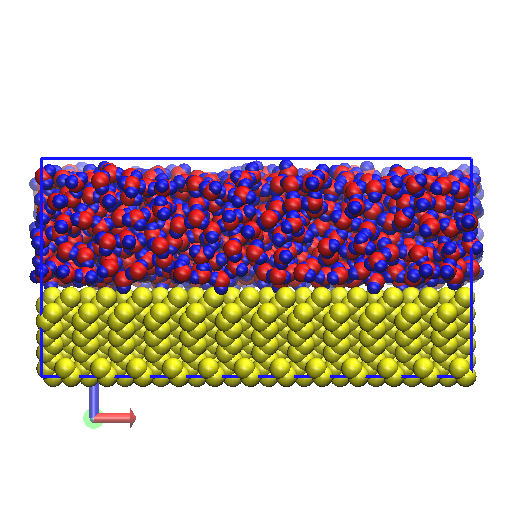
\includegraphics[width=95mm]{0pc_planar}
}
\subfloat{
  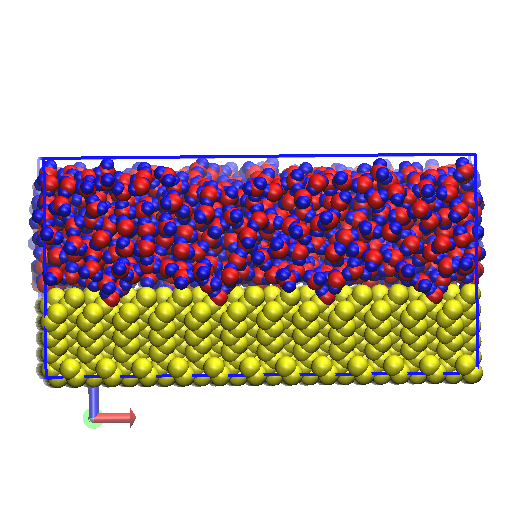
\includegraphics[width=95mm]{11pc_planar}
}
\newline
\subfloat{
  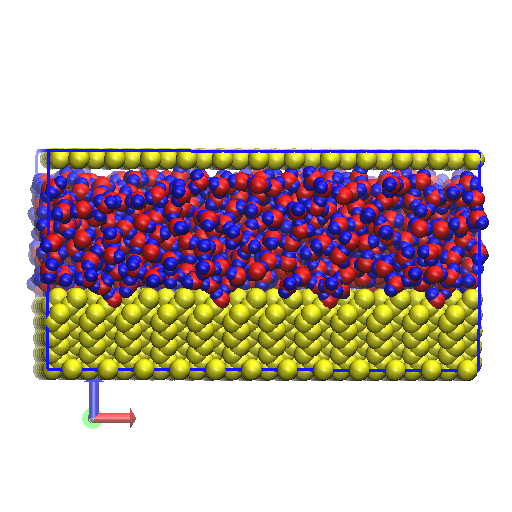
\includegraphics[width=95mm]{22pc_planar}
}
\subfloat{
  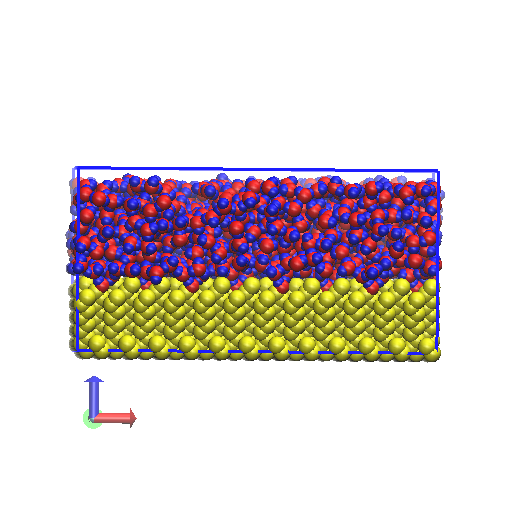
\includegraphics[width=95mm]{33pc_planar}
}
\newline
\subfloat{
  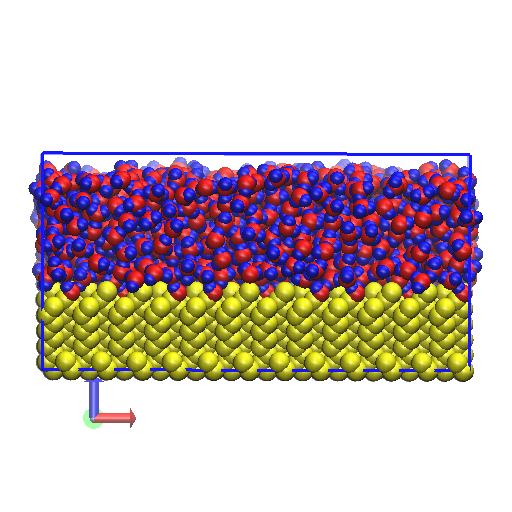
\includegraphics[width=95mm]{37pc_planar}
}
\subfloat{
  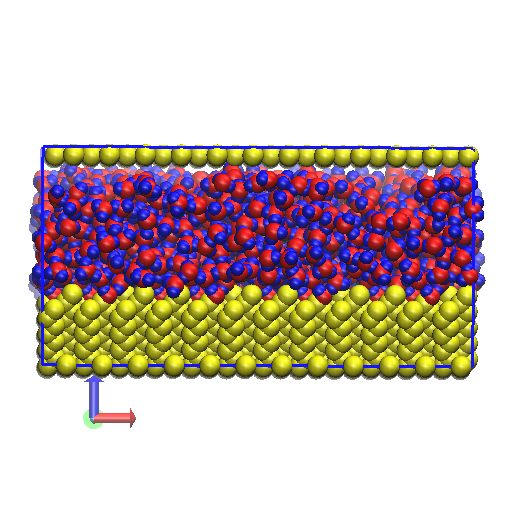
\includegraphics[width=95mm]{44pc_planar}
}
\end{figure}
\pagebreak

\begin{figure}
\subfloat{
  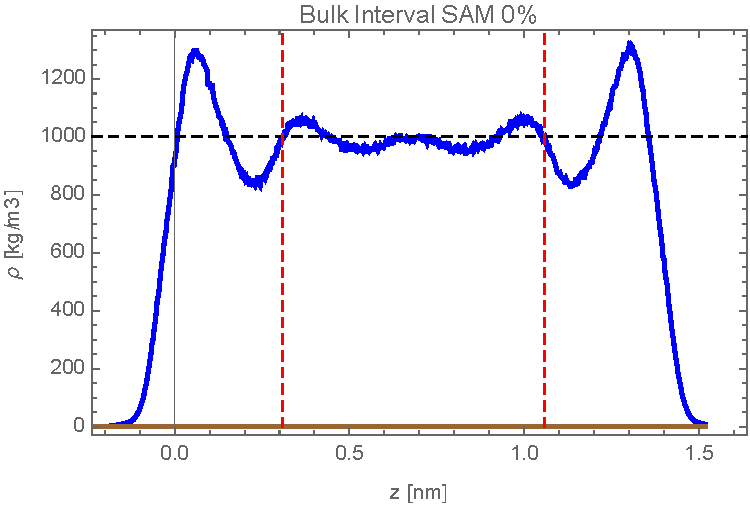
\includegraphics[width=95mm]{s0_bulk_interval}
}
\subfloat{
  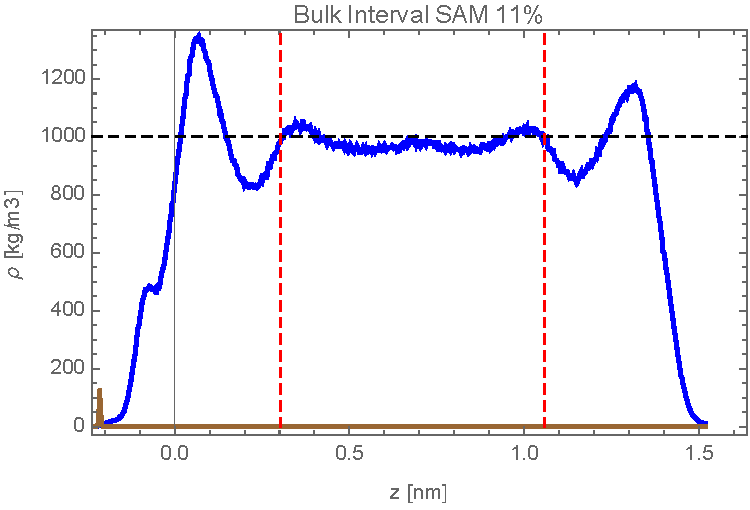
\includegraphics[width=95mm]{s11_bulk_interval}
}
\newline
\subfloat{
  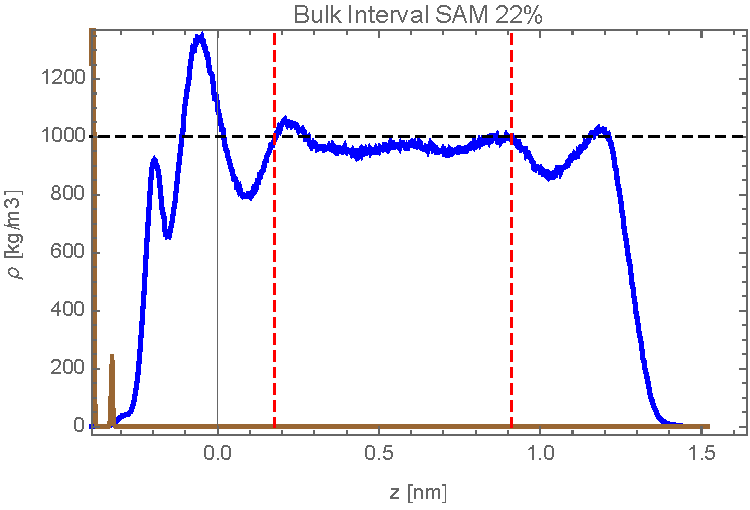
\includegraphics[width=95mm]{s22_bulk_interval}
}
\subfloat{
  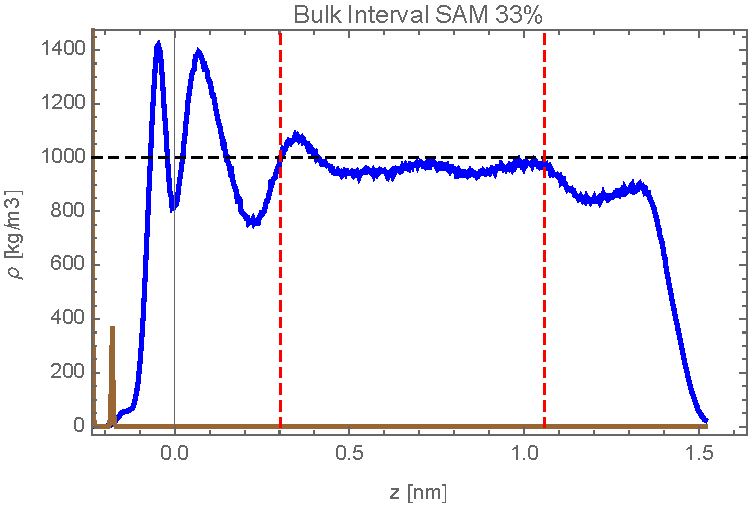
\includegraphics[width=95mm]{s33_bulk_interval}
}
\newline
\subfloat{
  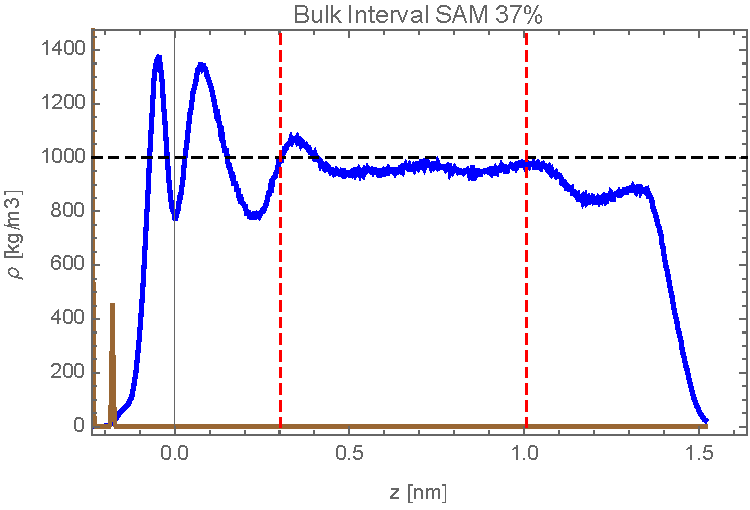
\includegraphics[width=95mm]{s37_bulk_interval}
}
\subfloat{
  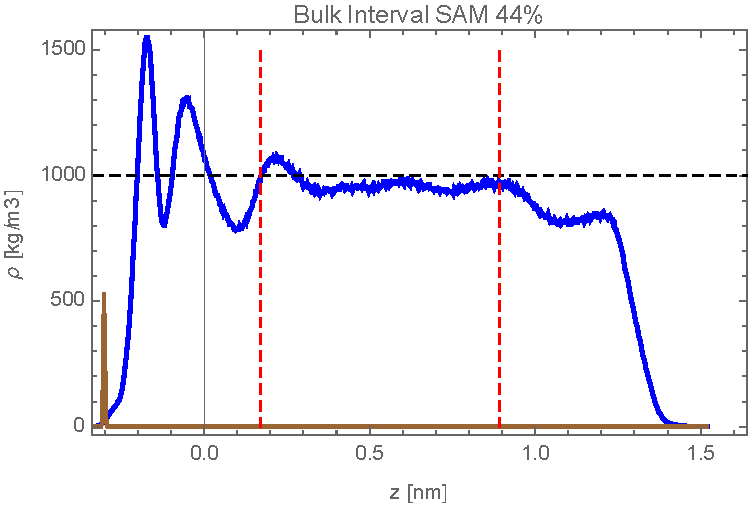
\includegraphics[width=95mm]{s44_bulk_interval}
}
\end{figure}
\pagebreak

\begin{figure}
\subfloat{
  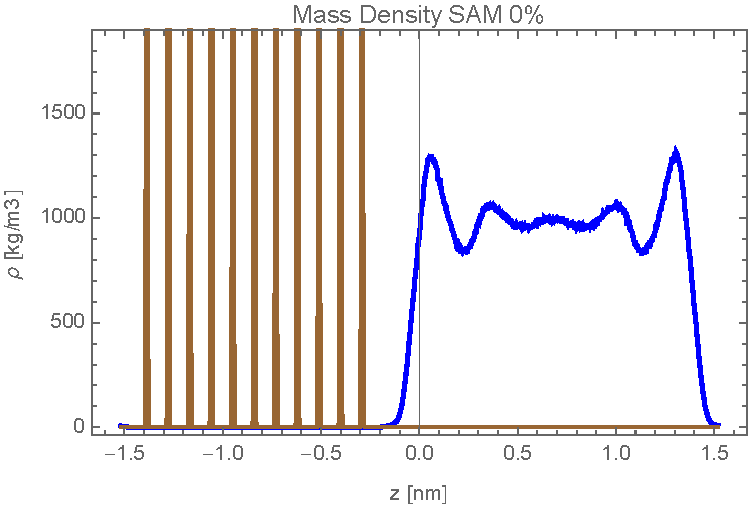
\includegraphics[width=95mm]{s0_all}
}
\subfloat{
  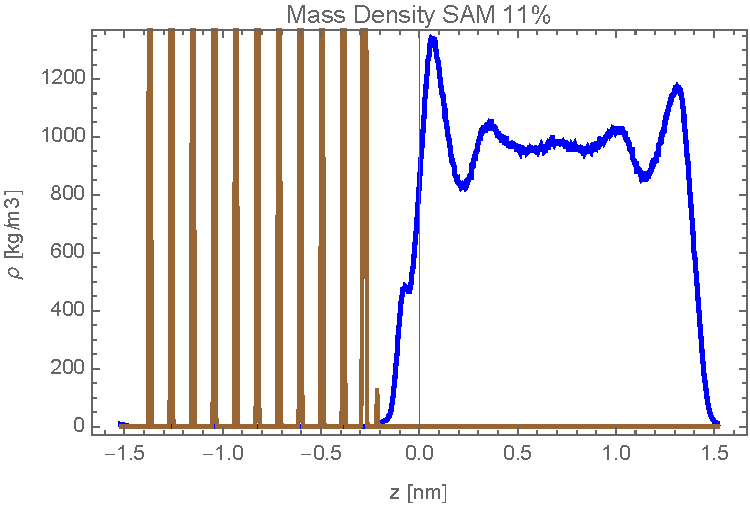
\includegraphics[width=95mm]{s11_all}
}
\newline
\subfloat{
  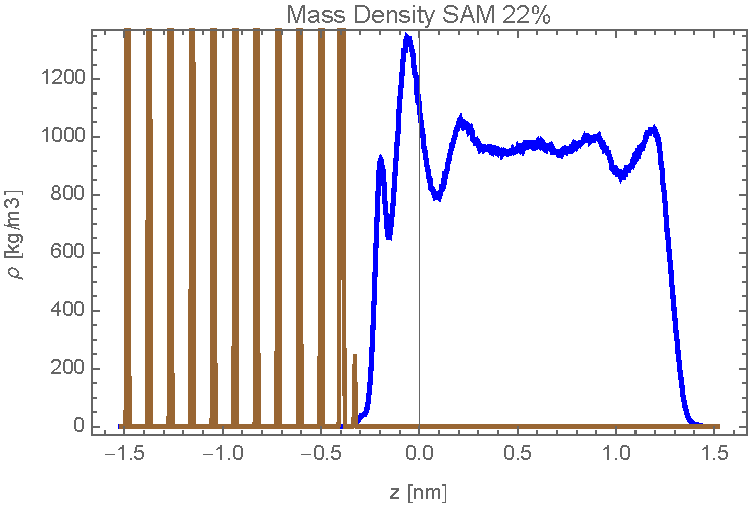
\includegraphics[width=95mm]{s22_all}
}
\subfloat{
  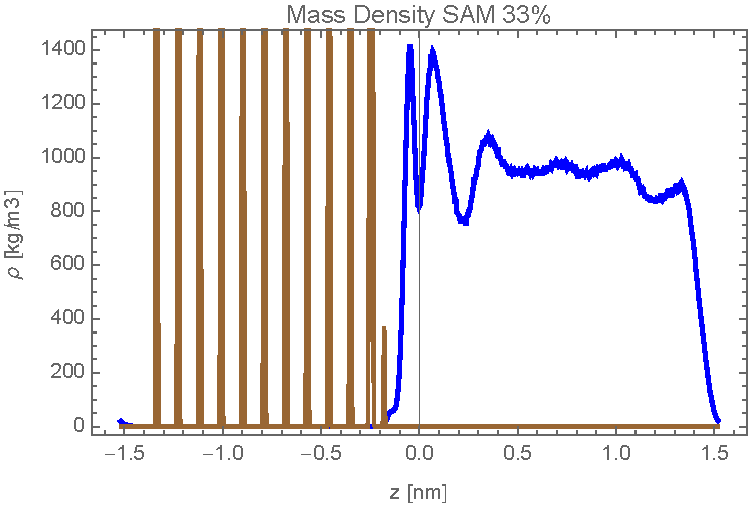
\includegraphics[width=95mm]{s33_all}
}
\newline
%\centering
\subfloat{
  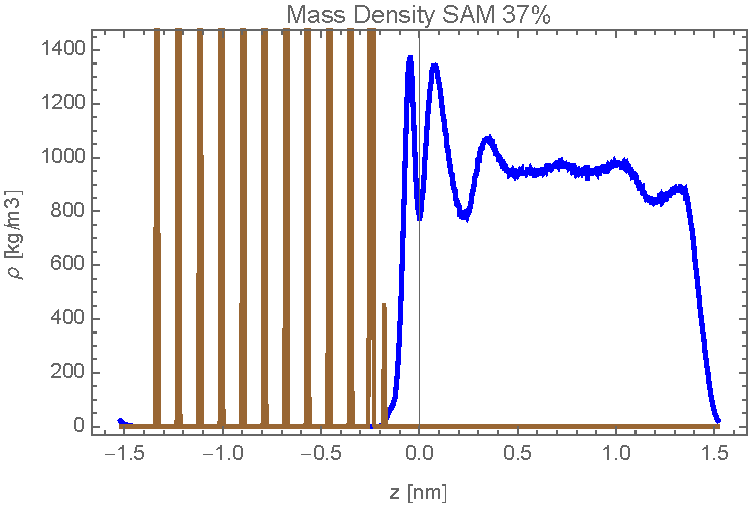
\includegraphics[width=95mm]{s37_all}
}
\subfloat{
  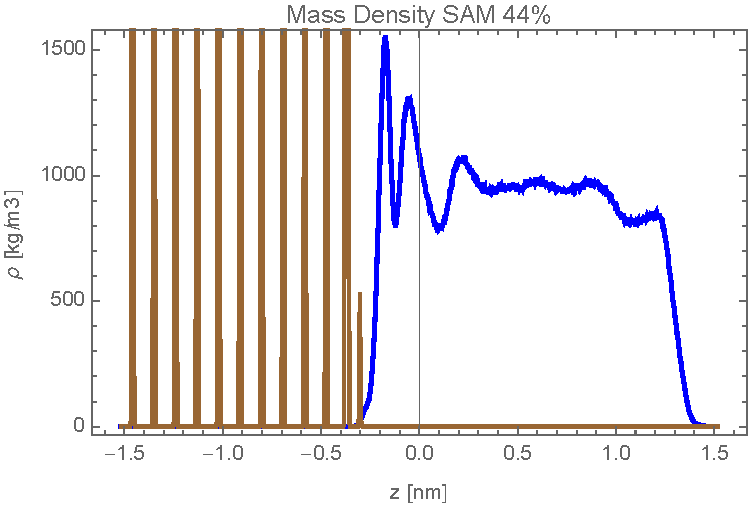
\includegraphics[width=95mm]{s44_all}
}
\end{figure}

\end{document}

